\chapter{Projekt aplikacji}

\section{Architektura}

Architektura aplikacji jest złożona z części mobilnej oraz czterech rozproszonych serwisów, z czego każdy występuje jako autonomiczna aplikacja z którą porozumiewanie odbywa się za pomocą protokołu HTTP. Warstwa prezentacyjna, porozumiewając się z pozostałymi serwisami zapewnia użytkownikowi płynną interakcję z systemem w celu osiągnięcia zamierzonych akcji dostępnych w obrębie funkcjonalności.\\
W ten sposób każda składowa część aplikacji może być niezależnie zarządzana. W momencie w którym pojedynczy element odpowiedzialny za szczególną usługę jest wyłączony, sama aplikacja może dalej działać wyłączając tylko funkcjonalności dostarczane przez niedostępny aktualnie serwis.\\
\linebreak
Takie podejście można określić mianem zorientowanym na usługi. Oznacza to, że przy tworzeniu systemu, spory nacisk kładziony jest na definiowanie spełniających wymagania użytkownika usług. Są one elementami oprogramowania zdolnymi do niezależnego funkcjonowania, udostępniającymi realizowane funkcje poprzez zdefiniowany interfejs.\\
\linebreak
HTTP (\texttt{Hypertext Transfer Protocol}), czyli ``Protokół Przesyłania Danych Hipertekstowych to protokół warstwy aplikacji, odpowiedzialny za transmisję dokumentów hipermedialnych, jak np. HTML. Został stworzony do komunikacji pomiędzy przeglądarkami, a serwerami webowymi, ale może być używany również w innych celach. HTTP opiera się na klasycznym modelu klient-serwer, gdzie klient inicjuje połączenie poprzez wysłanie żądania, następnie czeka na odpowiedź. HTTP jest protokołem bezstanowym, co oznacza, że serwer nie przechowuje żadnych danych (stanów) pomiędzy oboma żądaniami. (...)``\cite{http}
\linebreak

\begin{figure}[H]
	\centering
	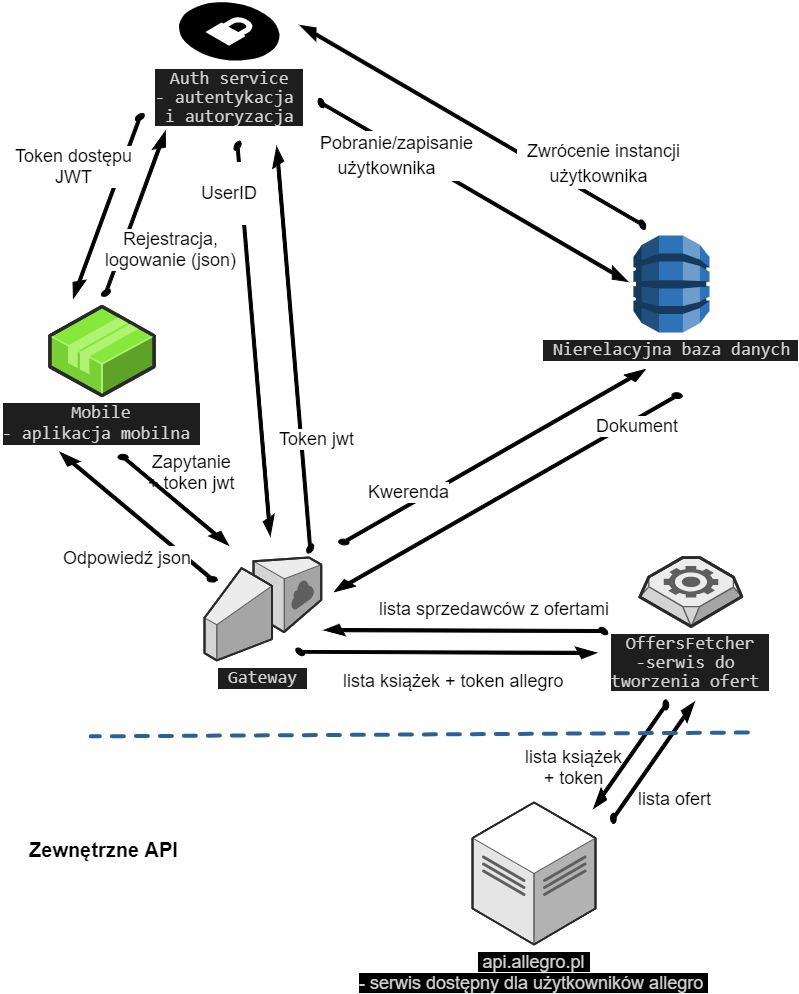
\includegraphics[width=\linewidth]{architecture_overview.png}
	\caption{Struktura systemu}
\end{figure}

\section{Auth service}
Auth service dba o zachowanie bezpieczeństwa w całym systemie.
Poprzez ekstrakcję funkcjonalności związanej z tworzeniem kont, logowaniem oraz zarządzaniem dostępem do pozostałych sektorów, gwarantuje niezawodną autentykację i autoryzację użytkownika pragnącego korzystać z aplikacji.\\
Informacje o kontach użytkowników przechowywane są w bazie danych, do której dostęp uzyskać można tylko za pomocą wygenerowanego przez nią, wewnętrznego klucza. 
\\
W celu swobodnego poruszania się po aplikacji należy uzyskać JWT(\texttt{JSON Web Token}). Aby pozsykać token należy się zarejestrować lub zalogować na ekranie logowania. Zapytanie utworzone w ten sposób zostanie wysłane do Auth service. W odpowiedzi przesłany zostanie wyżej wymieniony klucz dostępowy.\\

\subsection{JSON Web Token}

JSON Web Token to otwarty standard, który definiuje kompaktowy i samodzielny sposób na bezpieczny transfer danych. Poszczególna instancja składa się z trzech części oddzielonych kropkami w bezpośrednim formacie xx..x.y..yy.zz..z, gdzie poszczególne człony reprezentują: \cite{jwt}
\begin{enumerate}%[1)]
	\item Header - nagłówek, zawierający dwie informacje:
		\begin{itemize}
			\item typ tokenu, w tym przypadku "JWT"
			\item algorytm szyfrujący(n.p. HMAC, SHA256 lub RSA)
		\end{itemize}

	\item Payload - lista wyrażeń opisujących szyfrowaną informację, w przypadku użytkownika - np jego login, czy email.
	
	\item Signature - podpis stworzony poprzez zaszyfrowanie podanym w headerze algorytmem szyfrującym ciągu składającego się z
	\begin{itemize}
		\item zakodowanego za pomocą Base64 (specjalnego kodowania transportowego) nagłówka i listy wyrażeń
		\item sekretu, czyli unikalnego dla danych klucza.
	\end{itemize}
	\end{enumerate}

	\begin{figure}[H]
		\centering
		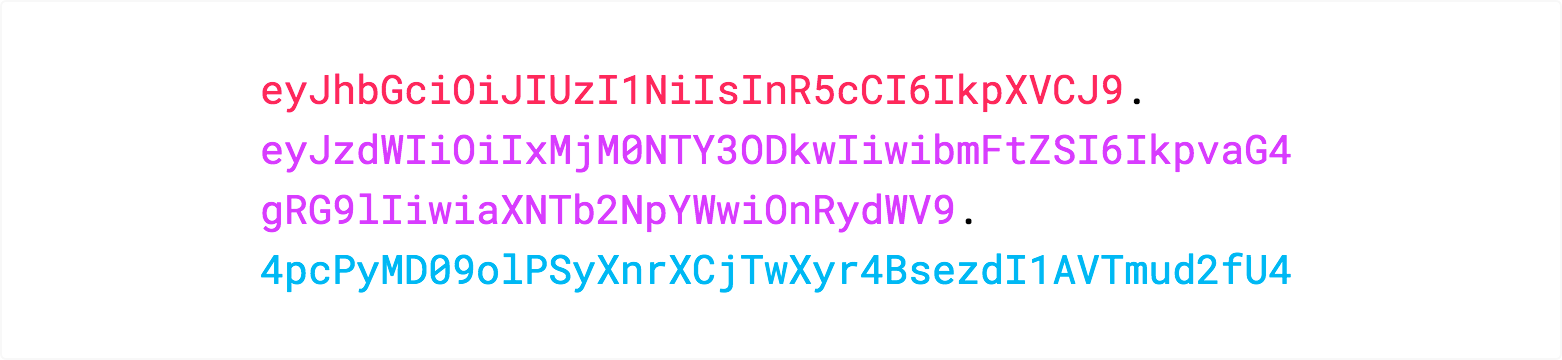
\includegraphics[width=\linewidth]{json-token.png}
		\caption{Przykładowy token jwt \cite{jwt}}
	\end{figure}

\subsection{Autoryzacja, a autentykacja}

Warto implicite rozróżnić dwa bardzo ważne pojęcia związane z bezpieczeństwem aplikacji ze względu na częstotliwość z jaką są one mylone.

\textbf{Autentykacja} - często też w dwóch częściach jako identyfikacja i uwierzytelnienie. Polega na potwierdzeniu tożsamości, to znaczy określeniu, czy podmiot procesu jest tym za kogo się podaje. Na przypadku logowania, strona ufająca otrzymuje od użytkownika podstawue stwierdza, czy użytkownik może być pozytywnie zweryfikowany.

\textbf{Autoryzacja} to potwierdzenie, czy dany użytkownik jest uprawniony do skorzystania z konkretnego zasobu. Na tym etapie autentykacja została ewaluowana pozytywnie. Nie oznacza to jednak, że dany podmiot posiada dostęp w żądanym zakresie. 


\section{Gateway}
Gateway to serwis zbudowany według podejścia zwanego \texttt{wzorcem bramy interfejsu API}\cite{api_gateway}. Jest to element znajdujący się pomiędzy klientem a rozproszonymi usługami. Dzięki temu w prosty sposób można kontrolować wszelkie zapytania skierowane do poszczególnych serwisów.\\
Jest to więc centralny punkt systemu, który ma na celu uproszczenie komunikacji warstwy prezentacyjnej z poszczególnymi usługami. Każde zapytanie wysłane do bramy zostaje zweryfikowane pod względem bezpieczeństwa. Następnie w zależności od potrzeb, modyfikowane, lub bezpośrednio przesłane dalej.
\begin{figure}[H]
	\centering
	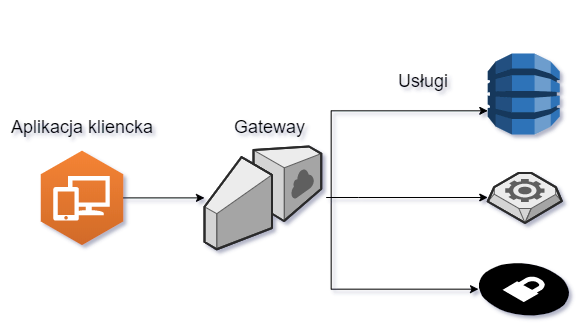
\includegraphics[width=\linewidth]{gateway.png}
	\caption{Gateway - schemat}
\end{figure}

\section{OffersFetcher}
OffersFetcher to główna jednostka licząca w systemie. Usługa ta otrzymuje żądanie z listą książek oraz token dostępowy do REST API portalu Allegro. (3.5.)
Dla każdej książki wykonywane jest odpowiednio zmodyfikowane zapytanie, którego rezultat jest przetwarzany i odkładany do odpowiedniej kolekcji, aby na koniec zostać wkomponowanym w pożądany rezultat. Analizowane są wszystkie obecnie dostępne w czasie rzeczywistym oferty sprzedaży w serwisie Allegro.pl. \\Dane otrzymane w ten sposób są przetwarzane i grupowane po unikalnym identyfikatorze sprzedawcy. Serwis zwraca odpowiedź w postaci listy zbiorów przedmiotów, które wpisują się w pozyzcje otrzymane w zapytaniu. 
\begin{figure}[H]
	\centering
	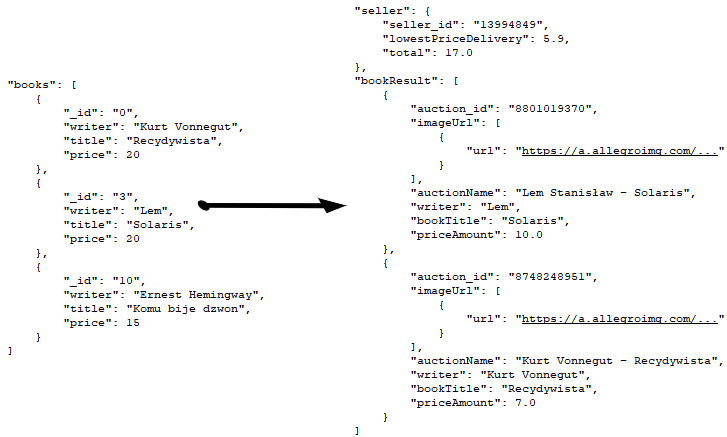
\includegraphics[width=\linewidth]{booksToOffers.png}
	\caption{Poszukiwane książki i bazująca na nich przykładowa oferta}
\end{figure}
\section{Zewnętrzne API}
Źródłem danych dla ofert tworzonych w serwisie OffersFetcher (3.4.)
jest Allegro REST API udostępnione przez Allegro.pl, czyli platformę transakcyjną on-line przedsiębiorstwa Allegro.pl. Portal ten umożliwa użytkownikom wystawianie na sprzedaż posiadanych przez nich przedmiotów oraz na korzystanie z ofert innych sprzedawców.\\
``Allegro REST API działa w oparciu o protokół HTTP (...) Autoryzacja realizowana jest w standardzie OAuth2.``\cite{allegroApi}\\ \newpage
\textbf{REST API} (\textbf{RE}presentational \textbf{S}tate \textbf{T}ransfer) to styl architektury oprogramowania w którym dane i funkcjonalności są odzwierciedlone  poprzez Ujednolicone Identyfikatory Zasobów(w skrócie URI). Termin ten został stworzony przez Roy Fielding w 2000 roku\cite{fielding}.Dostęp uzyskiwany jest poprzez proste i jasno zdefiniowane operacje. \linebreak Istnieje pięc obowiązkowych ograniczeń, które dokładnie definiują charakter tego podejścia:
\begin{itemize}
	\item bezstanowość - każde zapytanie do serwera powinno zawierać wszystkie informacje potrzebne do jego zrozumienia.
	\item użycie buforownia podręcznego - jeżeli dane są lokalnie przechowywane, należy o tym bezpośrednio poinformować.
	\item system warstwowy - istnieje możliwość użycia wielu komponentów do poszczególnych funkcjolności, które razem stanowią jedno API. Klient przeważnie nie jest w stanie określić, czy jego połączenie jest realizowane z serwerem końcowym czy którymś z pośredników.
	\item rozdział klienta od serwera - obie części powinno się być w stanie rozwijać osobno i niezależnie. Klient powinien jedynie znać URI, które może odpytywać.
	\item ujednolicony interfejs - należy deterministycznie zdefiniować i nie zmieniać adresów pod którymi dostępne będą zasoby. 
\end{itemize}
\cite{rest}

\section{Baza danych}
Warstwa persystencyjna jako osobny i niezależny serwis ma zadanie utrzymywać stan aplikacji. Jest to ogromnie ważny element systemu, którego działanie niezbędne jest np dla Auth service(3.2) ze względu na posiadane informacje o użytkownikach, które używane są w celu autoryzacji i autentykacji.
Oprócz danych dostępowych, dla każdego klienta przechowywane są również zbiory książek - posiadanych i poszukiwanych.\linebreak

Bazy danych można podzielić ze wględu na struktruę organizacji danych, którymi się kierują. Są to między innymi  
\section{Aplikacja mobilna}